\documentclass[12pt,a4paper]{article}

% ============================================================
% PACKAGES
% ============================================================
\usepackage[
    a4paper,
    top=1.55cm,
    bottom=1.35cm,
    left=1.75cm,
    right=1.75cm
]{geometry}

\usepackage[T1]{fontenc}
\usepackage{newtxtext}
\usepackage{graphicx}
\usepackage{xcolor}
\usepackage{array}
\usepackage{tabularx}
\usepackage{fancyhdr}
\usepackage{tikz}
\usepackage{eso-pic}
\usepackage{ragged2e}

% ============================================================
% COLORS
% ============================================================
\definecolor{GEUBlue}{RGB}{43,91,145}
\definecolor{GEUBannerBlue}{RGB}{0,102,148}
\definecolor{GEUYellow}{RGB}{255,201,38}
\definecolor{InstructionGrey}{RGB}{125,125,125}

% ============================================================
% GENERAL SETTINGS
% ============================================================
\setlength{\parindent}{0pt}
\setlength{\parskip}{0pt}
\renewcommand{\arraystretch}{1}

% ============================================================
% HEADER / FOOTER
% ============================================================
\pagestyle{fancy}
\fancyhf{}

\fancyhead[L]{%
    \fontsize{10.5}{12}\selectfont
    BTECH CSE DSCPP-III-2026-T278
}

\fancyhead[R]{%
    \fontsize{10.5}{12}\selectfont
    PHASE-II PROJECT PROGRESS
}

\fancyfoot[R]{%
    \fontsize{10}{12}\selectfont
    Page \thepage
}

\renewcommand{\headrulewidth}{0pt}
\renewcommand{\footrulewidth}{0pt}

\setlength{\headheight}{20pt}
\setlength{\headsep}{0.65cm}
\setlength{\footskip}{0.65cm}

% ============================================================
% BOTTOM YELLOW LINE
% ============================================================
\AddToShipoutPictureBG{%
\begin{tikzpicture}[remember picture,overlay]
    \fill[GEUYellow]
    (current page.south west)
    rectangle
    ([yshift=0.14cm]current page.south east);
\end{tikzpicture}
}

% ============================================================
% CUSTOM COMMANDS
% ============================================================
\newcommand{\sectiontitle}[1]{%
    {\color{GEUBlue}
    \fontsize{18}{22}\selectfont #1}
}

\newcommand{\instruction}[1]{%
    {\color{InstructionGrey}
    \fontsize{10.5}{13}\selectfont #1}
}

\newcommand{\answerbox}[2]{%
    \begin{tabularx}{\textwidth}{
        |>{\raggedright\arraybackslash}X|}
        \hline
        \parbox[t][#1][t]{\dimexpr\linewidth-12pt\relax}{
            \vspace{5pt}
            \fontsize{11}{13}\selectfont #2
        }\\
        \hline
    \end{tabularx}
}

% ============================================================
% DOCUMENT
% ============================================================
\begin{document}

% ============================================================
% PAGE 1
% ============================================================

\vspace*{0.10cm}

% Upload Graphic Era logo as geulogo.png
\includegraphics[width=8.0cm]{geulogo.png}

\vspace{0.70cm}

\noindent
\colorbox{GEUBannerBlue}{%
\parbox{\dimexpr\textwidth-2\fboxsep\relax}{
    \vspace{0.17cm}
    {\color{GEUYellow}
    \fontsize{16.5}{20}\selectfont
    \bfseries
    PROJECT AND TEAM INFORMATION}
    \vspace{0.17cm}
}}

\vspace{0.80cm}

% PROJECT TITLE
\sectiontitle{Project Title}

\vspace{0.05cm}

\instruction{}

\vspace{0.40cm}

\answerbox{1.00cm}{RouteLens: Live-Traffic Multiple Routes Visualization and Optimization System}

\vspace{0.80cm}

\noindent
\begin{tabularx}{\textwidth}{|>{\RaggedRight\arraybackslash}p{0.69\textwidth}|>{\RaggedRight\arraybackslash}X|}
\hline
\begin{minipage}[t]{\linewidth}
\vspace{1.5mm}
\textit{Team Name:}\\[-1mm]
\textit{Team \#}
\vspace{1.5mm}
\end{minipage}
&
\begin{minipage}[t]{\linewidth}
\vspace{1.5mm}
\textit{Carpe Diem}\\
\textit{DSCPP-III-2026-T278}
\vspace{1.5mm}
\end{minipage}
\\
\hline
\begin{minipage}[t][3.25cm][t]{\linewidth}
\vspace{1.5mm}
\textbf{Team member 1 (Team Lead)}\\[-1mm]
\textit{(Last Name, name: student ID: email, picture):}
\vspace{2.0cm}
\end{minipage}
&
\begin{minipage}[t][3.25cm][t]{\linewidth}
\vspace{1.5mm}
\textit{Upreti, Gunjita -- 2510382973}\\
\textit{2510382973@geu.ac.in}

\vspace{2mm}
\includegraphics[width=3.0cm,height=1.5cm,keepaspectratio]{gunjita.jpeg.png}
\end{minipage}
\\
\hline
\begin{minipage}[t][3.25cm][t]{\linewidth}
\vspace{1.5mm}
\textbf{Team member 2}\\[-1mm]
\textit{(Last Name, name: student ID: email, picture):}
\vspace{2.0cm}
\end{minipage}
&
\begin{minipage}[t][3.25cm][t]{\linewidth}
\vspace{1.5mm}
\textit{Rawat, Sneha -- 2510012141}\\
\textit{2510012141@geu.ac.in}

\vspace{2mm}
\includegraphics[width=3.0cm,height=1.5cm,keepaspectratio]{sneha.jpeg.png}
\end{minipage}
\\
\hline
\begin{minipage}[t][3.25cm][t]{\linewidth}
\vspace{1.5mm}
\textbf{Team member 3}\\[-1mm]
\textit{(Last Name, name: student ID: email, picture):}
\vspace{2.0cm}
\end{minipage}
&
\begin{minipage}[t][3.25cm][t]{\linewidth}
\vspace{1.5mm}
\textit{Rawat, Aayush -- 2510370528}\\
\textit{2510370528@geu.ac.in}

\vspace{2mm}
\includegraphics[width=3.0cm,height=1.5cm,keepaspectratio]{aayush.jpeg.png}
\end{minipage}
\\
\hline
\end{tabularx}

\newpage
% ============================================================
% PAGE 2
% ============================================================

\vspace*{0.15cm}

\noindent
\colorbox{GEUBannerBlue}{%
\parbox{\dimexpr\textwidth-2\fboxsep\relax}{
    \vspace{0.18cm}
    {\color{GEUYellow}
    \fontsize{17}{21}\selectfont
    \bfseries
    PHASE-II PROJECT PROGRESS DESCRIPTION (35 pts)}
    \vspace{0.18cm}
}}

\vspace{0.70cm}

% PROJECT ABSTRACT
\sectiontitle{Project Abstract (2 pts)}

\vspace{0.05cm}

\instruction{

}

\vspace{0.12cm}

\answerbox{7.25cm}{RouteLens is a web-based route planning system that helps commuters choose between several driving routes by showing them together on one map and comparing them on more than travel time. For a chosen start point and destination, it generates up to three genuinely different routes over the real road network of Dehradun, draws each route in a distinct colour, and attaches an information box with the estimated time of arrival (ETA), distance, number of traffic signals and a Low/Medium/High traffic level. The recommended route is highlighted with a short explanation of why it was preferred.

\vspace{6pt}
Following the Phase-I review, the project no longer uses an imaginary map or simulated traffic. The road graph is built from real OpenStreetMap (OSM) data, and live traffic speeds come from the TomTom Traffic Flow API through API keys stored only on the server. When live data is unavailable, the system falls back to free-flow travel times and informs the user.

\vspace{6pt}
The core is written in C++ using a directed adjacency-list graph, a hand-written binary min-heap for Dijkstra's algorithm and A$^{*}$ search, the penalty method and Yen's algorithm for alternative routes, a KD-tree for nearest-road lookup and an LRU cache for traffic data. Users can adjust their priorities (time, distance, signals, congestion), making the comparison a transparent decision aid rather than a single fixed answer.}

\vspace{0.70cm}

% UPDATED PROJECT APPROACH
\sectiontitle{Updated Project Approach and Architecture (2 pts)}

\vspace{0.05cm}

\instruction{
}

\vspace{0.25cm}

\answerbox{11.60cm}{\textbf{System design.} RouteLens uses a three-tier client--server design.
(1) \textit{Offline data layer:} a Python script using OSMnx extracts the drivable OSM network of Dehradun and exports nodes, directed edges (length, road class, free-flow speed), road geometry and traffic-signal tags to CSV files.
(2) \textit{C++17 backend:} builds a directed adjacency-list graph (hash map for OSM-ID mapping), keeps the largest strongly connected component (iterative Tarjan's algorithm) and snaps clicked points to the nearest node with a KD-tree. Routes are computed with Dijkstra's algorithm and A$^{*}$ on a self-written binary min-heap; alternatives come from the penalty method and Yen's $k$-shortest paths, filtered by overlap and stretch, then ranked by a Pareto filter and a user-weighted score. The Traffic Manager samples points along candidate routes, queries the TomTom Traffic Flow Segment Data API and updates the speed ratio of each matched edge, using an LRU cache (hash map + doubly linked list, 5-minute expiry) and a queue-based rate limiter.
(3) \textit{Web frontend:} HTML, CSS and JavaScript with Leaflet.js for the map and Chart.js for route comparison.

\vspace{5pt}
\textbf{Communication protocols.} JSON over HTTP REST endpoints (\texttt{/api/routes}, \texttt{/api/health}, \texttt{/api/traffic/status}) between browser and server; HTTPS from the server to TomTom. The API key is read from an environment variable and never reaches the browser.

\vspace{5pt}
\textbf{Libraries and tools.} Crow (web server), cpp-httplib with OpenSSL (HTTPS client), nlohmann/json, SQLite, GoogleTest, OSMnx, Leaflet.js, Chart.js; CMake, Git/GitHub and GitHub Actions CI.

\vspace{6pt}
{\centering
\begin{tikzpicture}[
    every node/.style={draw, rounded corners=2pt, align=center,
        text width=2.85cm, minimum height=1.0cm, font=\scriptsize},
    >=stealth]
    \node (ui)  at (0,0)       {\textbf{Web Frontend}\\HTML/CSS/JS,\\Leaflet, Chart.js};
    \node (api) at (4.3,0)     {\textbf{C++ REST Server}\\(Crow)\\/api/routes};
    \node (tm)  at (8.6,0)     {\textbf{Traffic Manager}\\LRU cache,\\rate-limit queue};
    \node (tt)  at (12.9,0)    {\textbf{TomTom Traffic}\\Flow API};
    \node (rm)  at (4.3,-1.75) {\textbf{Route Manager}\\Dijkstra, A$^{*}$, penalty,\\Yen's, scoring};
    \node (g)   at (8.6,-1.75) {\textbf{Graph + KD-tree}\\adjacency list,\\SCC cleaning};
    \node (osm) at (12.9,-1.75){\textbf{OSM data}\\OSMnx $\rightarrow$\\nodes/edges CSV};
    \draw[<->, thick] (ui) -- node[draw=none, above, text width=1.1cm, inner sep=1pt, minimum height=0pt, font=\tiny]{JSON/\\HTTP} (api);
    \draw[<->, thick] (tm) -- node[draw=none, above, text width=1.1cm, inner sep=1pt, minimum height=0pt, font=\tiny]{HTTPS\\+ API key} (tt);
    \draw[->, thick] (api) -- (rm);
    \draw[<->, thick] (rm) -- (g);
    \draw[<->, thick] (rm) -- (tm);
    \draw[->, thick] (tm) -- node[draw=none, right, text width=1.4cm, inner sep=2pt, minimum height=0pt, font=\tiny]{speed ratios} (g);
    \draw[->, thick] (osm) -- (g);
\end{tikzpicture}
\par}}

\newpage

% ============================================================
% PAGE 3
% ============================================================

\vspace*{0.20cm}

% TASKS COMPLETED
\sectiontitle{Tasks Completed (7 pts)}

\vspace{0.05cm}

\instruction{

}

\vspace{0.20cm}

\begin{tabularx}{\textwidth}{
|>{\raggedright\arraybackslash}X
|>{\raggedright\arraybackslash}X|
}
\hline
\textbf{Task Completed} &
\textbf{Team Member}\\
\hline

\parbox[t]{\linewidth}{\raggedright\fontsize{11}{13}\selectfont\strut OSM data pipeline: OSMnx extraction of the Dehradun road network; export of nodes, directed edges, geometry and signal tags; C++ CSV loader with hash-map ID mapping; largest-SCC cleaning (iterative Tarjan).\strut}
&
\parbox[t]{\linewidth}{\raggedright\fontsize{11}{13}\selectfont\strut Sneha Rawat\strut}
\\
\hline

\parbox[t]{\linewidth}{\raggedright\fontsize{11}{13}\selectfont\strut Hand-written binary min-heap; Dijkstra's algorithm and A$^{*}$ search with lazy deletion; unit tests against reference shortest-path results.\strut}
&
\parbox[t]{\linewidth}{\raggedright\fontsize{11}{13}\selectfont\strut Gunjita Upreti\strut}
\\
\hline

\parbox[t]{\linewidth}{\raggedright\fontsize{11}{13}\selectfont\strut Alternative routes: penalty method, Yen's $k$-shortest paths, overlap and stretch filtering; Pareto filter, weighted scoring and route explanation text.\strut}
&
\parbox[t]{\linewidth}{\raggedright\fontsize{11}{13}\selectfont\strut Gunjita Upreti\strut}
\\
\hline

\parbox[t]{\linewidth}{\raggedright\fontsize{11}{13}\selectfont\strut KD-tree nearest-node snapping; edge-geometry loading so routes follow real road curves.\strut}
&
\parbox[t]{\linewidth}{\raggedright\fontsize{11}{13}\selectfont\strut Sneha Rawat\strut}
\\
\hline

\parbox[t]{\linewidth}{\raggedright\fontsize{11}{13}\selectfont\strut TomTom Traffic Flow client with server-side API key; LRU cache with expiry; queue-based rate limiter; segment-to-edge matching; ETA, traffic-level and signal-count computation; free-flow fallback.\strut}
&
\parbox[t]{\linewidth}{\raggedright\fontsize{11}{13}\selectfont\strut Sneha Rawat\strut}
\\
\hline

\parbox[t]{\linewidth}{\raggedright\fontsize{11}{13}\selectfont\strut Crow REST server (\texttt{/api/routes}, \texttt{/api/health}, \texttt{/api/traffic/status}), JSON input validation and static website hosting.\strut}
&
\parbox[t]{\linewidth}{\raggedright\fontsize{11}{13}\selectfont\strut Aayush Rawat\strut}
\\
\hline

\parbox[t]{\linewidth}{\raggedright\fontsize{11}{13}\selectfont\strut Website: Leaflet map with draggable start/end markers, colour-coded routes with information boxes, highlighted recommended route, route cards, Chart.js comparison and priority sliders.\strut}
&
\parbox[t]{\linewidth}{\raggedright\fontsize{11}{13}\selectfont\strut Aayush Rawat\strut}
\\
\hline

\parbox[t]{\linewidth}{\raggedright\fontsize{11}{13}\selectfont\strut GitHub repository, CMake build, GitHub Actions CI, secure API-key handling (\texttt{.env} excluded via \texttt{.gitignore}); module integration.\strut}
&
\parbox[t]{\linewidth}{\raggedright\fontsize{11}{13}\selectfont\strut Aayush Rawat (repository, CI); Gunjita Upreti (integration)\strut}
\\
\hline
\end{tabularx}

\vspace{0.65cm}

% CHALLENGES
\sectiontitle{Challenges/Roadblocks (7 pts)}

\vspace{0.05cm}

\instruction{

}

\vspace{0.18cm}

\answerbox{8.30cm}{\textbf{1. Fitting live traffic onto our own graph.} TomTom reports traffic for its own road segments, not for our OSM edges, and querying every edge is impossible within the free limit of 2,500 non-tile requests per day. We sample points every 300--500\,m along candidate routes on major roads and match each returned segment to graph edges within about 20\,m and in a similar direction, using the KD-tree. An area-wide refresh with HERE's bounding-box flow API is planned to reduce calls further.

\vspace{4pt}
\textbf{2. API quota.} An LRU cache with 5-minute expiry, removal of duplicate sample points and a queue-based rate limiter keep usage low; daily calls and cache hit rate are monitored through \texttt{/api/traffic/status}.

\vspace{4pt}
\textbf{3. Incomplete real-world data.} Live coverage on minor roads is limited and many traffic signals are not tagged in OSM. Live data is applied only where the API's confidence is adequate, with a visible free-flow fallback elsewhere; signals on test routes are audited through a local overrides file.

\vspace{4pt}
\textbf{4. Near-duplicate alternatives.} Yen's algorithm tends to return routes differing only by a small detour, so the penalty method is the primary generator, with overlap and stretch filters on all candidates; thresholds will be tuned during evaluation.

\vspace{4pt}
\textbf{5. Engineering issues.} Tarjan's algorithm is written iteratively to avoid stack overflow on a large graph; a mutex and per-request weight copies prevent data races in the multithreaded server; the fixed signal delay is applied only in free-flow mode so that waiting time already included in live speeds is not counted twice.}

\vspace{0.65cm}

% TASKS PENDING
\sectiontitle{Tasks Pending (7 pts)}

\vspace{0.05cm}

\instruction{

}

\vspace{0.18cm}

\begin{tabularx}{\textwidth}{
|>{\raggedright\arraybackslash}X
|>{\raggedright\arraybackslash}X|
}
\hline

\textbf{Task Pending} &
\textbf{Team Member (to complete the task)}
\\
\hline

\parbox[t]{\linewidth}{\raggedright\fontsize{11}{13}\selectfont\strut Scenario (what-if) mode: block or slow selected roads, BFS reachability check, \texttt{/api/scenario} endpoint and its user interface.\strut}
&
\parbox[t]{\linewidth}{\raggedright\fontsize{11}{13}\selectfont\strut Gunjita Upreti (backend); Aayush Rawat (interface)\strut}
\\
\hline

\parbox[t]{\linewidth}{\raggedright\fontsize{11}{13}\selectfont\strut Traffic history logging in SQLite and departure-time comparison of routes.\strut}
&
\parbox[t]{\linewidth}{\raggedright\fontsize{11}{13}\selectfont\strut Sneha Rawat\strut}
\\
\hline

\parbox[t]{\linewidth}{\raggedright\fontsize{11}{13}\selectfont\strut Area-wide traffic refresh using the HERE Traffic API v7 (bounding-box flow) to reduce per-query API calls.\strut}
&
\parbox[t]{\linewidth}{\raggedright\fontsize{11}{13}\selectfont\strut Sneha Rawat\strut}
\\
\hline

\parbox[t]{\linewidth}{\raggedright\fontsize{11}{13}\selectfont\strut Algorithm evaluation: correctness on 1,000 random origin--destination pairs against NetworkX; Dijkstra vs.\ A$^{*}$; own heap vs.\ \texttt{std::priority\_queue}; penalty method vs.\ Yen's (overlap, stretch).\strut}
&
\parbox[t]{\linewidth}{\raggedright\fontsize{11}{13}\selectfont\strut Gunjita Upreti\strut}
\\
\hline

\parbox[t]{\linewidth}{\raggedright\fontsize{11}{13}\selectfont\strut ETA accuracy study against TomTom Routing ETAs and real timed trips; failure analysis.\strut}
&
\parbox[t]{\linewidth}{\raggedright\fontsize{11}{13}\selectfont\strut Sneha Rawat\strut}
\\
\hline

\parbox[t]{\linewidth}{\raggedright\fontsize{11}{13}\selectfont\strut Usability study with classmates; mobile layout and colour-blind accessibility; Docker-based deployment.\strut}
&
\parbox[t]{\linewidth}{\raggedright\fontsize{11}{13}\selectfont\strut Aayush Rawat\strut}
\\
\hline

\parbox[t]{\linewidth}{\raggedright\fontsize{11}{13}\selectfont\strut Final report, documentation, demo video and viva preparation.\strut}
&
\parbox[t]{\linewidth}{\raggedright\fontsize{11}{13}\selectfont\strut All members\strut}
\\
\hline

\end{tabularx}

\newpage

% ============================================================
% PAGE 4
% ============================================================

\vspace*{0.30cm}

% PROJECT OUTCOME
\sectiontitle{Project Outcome/Deliverables (2 pts)}

\vspace{0.05cm}

\instruction{

}

\vspace{0.35cm}

\answerbox{6.80cm}{The final deliverable is a working RouteLens website backed by a C++ routing engine, demonstrated on the real road network of Dehradun with live traffic data.

\vspace{5pt}
\textbf{1. Web application:} selection of start and destination by clicking or dragging markers; up to three colour-coded routes on one map, each with an information box (ETA, distance, traffic signals, traffic level); a highlighted recommended route with an explanation; adjustable priorities; and a what-if scenario mode.

\vspace{5pt}
\textbf{2. C++ routing engine:} hand-written data structures (adjacency-list graph, binary min-heap, KD-tree, LRU cache, queue, hash map) and algorithms (Dijkstra, A$^{*}$, penalty method, Yen's algorithm, Tarjan's SCC, BFS), exposed through a REST API.

\vspace{5pt}
\textbf{3. Live-traffic integration:} TomTom traffic data with server-side API keys, caching, rate limiting and free-flow fallback.

\vspace{5pt}
\textbf{4. Evaluation report:} correctness, performance, ETA-accuracy and usability results with failure analysis.

\vspace{5pt}
\textbf{5. Source code repository:} with unit tests, continuous integration, documentation and a demo video.}

\vspace{0.75cm}

% PROGRESS OVERVIEW
\sectiontitle{Progress Overview (2 pts)}

\vspace{0.05cm}

\instruction{

}

\vspace{0.25cm}

\answerbox{5.70cm}{\textbf{How much is done:} About \textbf{78\%} of the project is complete (Phase-II target: 75\%).

\vspace{5pt}
\textbf{What works now:} A user can click a start and end point on the website and get up to three routes calculated by our own C++ code, using real Dehradun roads and live TomTom traffic. Each route shows its ETA, distance, number of signals and traffic level, and the best route is highlighted.

\vspace{5pt}
\textbf{Ahead of schedule:} Priority sliders and route explanations, which were not in our Phase-I plan, are already working.

\vspace{5pt}
\textbf{Behind schedule:} Scenario mode (blocking or slowing a road) is not finished, because matching TomTom traffic data to our roads took longer than expected. It is our first task in Phase III.

\vspace{5pt}
\textbf{Still to do (about 22\%):} scenario mode, traffic history, testing and evaluation, user study, design polish, deployment and final documentation.}

\newpage

% ============================================================
% PAGE 5
% ============================================================

\vspace*{0.20cm}

% CODEBASE
\sectiontitle{Codebase Information (2 pts)}

\vspace{0.05cm}

\instruction{
}

\vspace{0.20cm}

\answerbox{6.65cm}{\textbf{Repository:} \textcolor{red}{[https://github.com/gunjita18/RouteLens-DSCPP]}.

\vspace{3pt}
\textbf{Branches:} \texttt{main} (stable, protected; merged only through reviewed pull requests), \texttt{dev} (integration) and \texttt{feature/*} branches. \textbf{Structure:} \texttt{preprocess/}, \texttt{src/\{graph, ds, routing, traffic, api\}}, \texttt{web/}, \texttt{tests/}.

\vspace{3pt}
\textbf{Important commits:}\\
\textcolor{red}{} -- CMake/Crow project skeleton and GitHub Actions CI\\
\textcolor{red}{} -- OSMnx export script and C++ graph loader with SCC cleaning\\
\textcolor{red}{} -- Binary min-heap, Dijkstra and A$^{*}$ with unit tests\\
\textcolor{red}{} -- Penalty method, Yen's algorithm and route filtering\\
\textcolor{red}{} -- TomTom traffic client, LRU cache and rate limiter\\
\textcolor{red}{} -- Leaflet frontend with multi-route display and comparison panel

\vspace{3pt}
\textbf{Security:} API keys are not stored in the repository; only \texttt{.env.example} is committed and \texttt{.env} is excluded through \texttt{.gitignore}.}

\vspace{0.65cm}

% TESTING
\sectiontitle{Testing and Validation Status (2 pts)}

\vspace{0.05cm}

\instruction{}

\vspace{0.30cm}

\begin{tabularx}{\textwidth}{
|>{\raggedright\arraybackslash}p{0.34\textwidth}
|>{\raggedright\arraybackslash}p{0.31\textwidth}
|>{\raggedright\arraybackslash}X|
}
\hline

\textbf{Test Type} &
\textbf{Status (Pass/Fail)} &
\textbf{Notes}
\\
\hline

\parbox[t]{\linewidth}{\raggedright\fontsize{10.5}{12.5}\selectfont\strut Unit tests (data structures)\strut}
&
\parbox[t]{\linewidth}{\raggedright\fontsize{10.5}{12.5}\selectfont\strut Pass\strut}
&
\parbox[t]{\linewidth}{\raggedright\fontsize{10.5}{12.5}\selectfont\strut Heap, KD-tree and cache checked on sample inputs.\strut}
\\
\hline

\parbox[t]{\linewidth}{\raggedright\fontsize{10.5}{12.5}\selectfont\strut Route correctness\strut}
&
\parbox[t]{\linewidth}{\raggedright\fontsize{10.5}{12.5}\selectfont\strut Pass\strut}
&
\parbox[t]{\linewidth}{\raggedright\fontsize{10.5}{12.5}\selectfont\strut Routes checked against a reference tool on sample trips.\strut}
\\
\hline

\parbox[t]{\linewidth}{\raggedright\fontsize{10.5}{12.5}\selectfont\strut Traffic API integration\strut}
&
\parbox[t]{\linewidth}{\raggedright\fontsize{10.5}{12.5}\selectfont\strut Pass\strut}
&
\parbox[t]{\linewidth}{\raggedright\fontsize{10.5}{12.5}\selectfont\strut Live traffic data received; free-flow fallback works.\strut}
\\
\hline

\parbox[t]{\linewidth}{\raggedright\fontsize{10.5}{12.5}\selectfont\strut Website (manual testing)\strut}
&
\parbox[t]{\linewidth}{\raggedright\fontsize{10.5}{12.5}\selectfont\strut Pass\strut}
&
\parbox[t]{\linewidth}{\raggedright\fontsize{10.5}{12.5}\selectfont\strut Routes and info boxes display correctly in the browser.\strut}
\\
\hline

\parbox[t]{\linewidth}{\raggedright\fontsize{10.5}{12.5}\selectfont\strut Performance and accuracy evaluation\strut}
&
\parbox[t]{\linewidth}{\raggedright\fontsize{10.5}{12.5}\selectfont\strut Pending\strut}
&
\parbox[t]{\linewidth}{\raggedright\fontsize{10.5}{12.5}\selectfont\strut Planned for Phase III.\strut}
\\
\hline

\end{tabularx}

\vspace{0.65cm}

% DELIVERABLES PROGRESS
\sectiontitle{Deliverables Progress (2 pts)}

\vspace{0.05cm}

\instruction{

}

\vspace{0.25cm}

\answerbox{3.90cm}{\textbf{1. Website} -- \textit{In progress.} Main features are working; scenario mode and design polish are pending.

\vspace{4pt}
\textbf{2. C++ routing engine} -- \textit{Mostly completed.} Scenario mode is pending.

\vspace{4pt}
\textbf{3. Live-traffic integration} -- \textit{Completed.}

\vspace{4pt}
\textbf{4. Traffic history} -- \textit{Pending.}

\vspace{4pt}
\textbf{5. Evaluation report} -- \textit{Pending} (Phase III).

\vspace{4pt}
\textbf{6. Code repository and documentation} -- \textit{In progress.}}

\end{document}
